%%%%%%%%%%%%%%%%%%%%%%%%%%%%%%%%%%%%%%%%%%%%%%%%%%%%%%%%%%%%%%%%%%%%%%%%
% Preamble
%%%%%%%%%%%%%%%%%%%%%%%%%%%%%%%%%%%%%%%%%%%%%%%%%%%%%%%%%%%%%%%%%%%%%%%%
\documentclass[12pt]{article}
%
% Packages and other includes
% Pagination
\usepackage[letterpaper, margin=1in]{geometry}
\usepackage{titling}
\setlength{\droptitle}{-5em}
%
% Graphics, floats, tables
\usepackage{graphicx, color, float, array}
\graphicspath{{image/}}
%
% Fonts
\usepackage[T1]{fontenc} % best for Western European languages
\usepackage{lmodern} % Latin Modern instead of CM
\usepackage{textcomp} % required to get special symbols
%
% Math
\usepackage{amsmath, amssymb}
\usepackage{enumerate}
\usepackage{braket}
% 
% Hyperlinks
\usepackage[colorlinks,linkcolor={red},citecolor={blue},
urlcolor={blue}]{hyperref} 
%
% Definitions and settings
% Paragraph indent and spacing
\setlength{\parskip}{0.4\baselineskip}
\setlength{\parindent}{0in}
%
% Math mode version of "r" column type (requires array package)
\newcolumntype{R}{>{$}r<{$}}
% Title, authors, date
\title{\textbf{Matter, Relative Atomic Mass, and Periodic Table}}
\date{Aug 31, 2022}
\renewcommand\maketitlehookc{\vspace{-10ex}}

\begin{document}

\maketitle 

\textbf{Matter Classification}

1) Determine whether each molecular diagram represents a pure substance or a
mixture. If it represents a pure substance, classify the substance as an
element or compound. If it represents a mixture, classify the mixture as
homogeneous or heterogeneous.

\begin{center}
  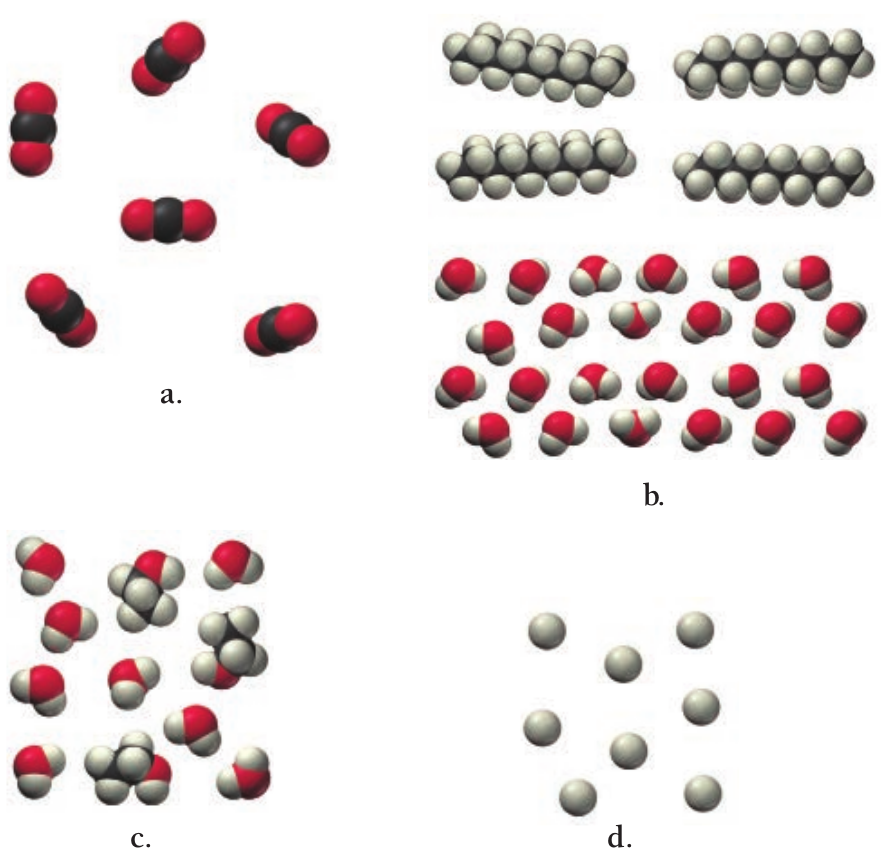
\includegraphics[scale=0.25]{matter_classify}
\end{center}


\textbf{Scientific Method}

2) Classify each statement as an observation, a law, or a theory.
\vspace{0in}
\begin{enumerate}[a)]
\itemsep0em
\item All matter is made of tiny, indestructible particles called
  atoms.
\item When iron rusts in a closed container, the mass of the container
  and its contents do not change.
\item In chemical reactions, matter is neither created nor destroyed
\item When a match burns, heat is released.
\item Chlorine is a highly reactive gas.
\item Neon is an inert (or nonreactive) gas.
\item The reactivity of elements depends on the arrangement of their
  electrons.
\end{enumerate}

\textbf{Relative Sizes}

3) The single proton that forms the nucleus of the hydrogen atom has
a readius of approximately $1.0\times 10^{-13}$ cm. The hydrogen atom itself
has a radius of approximately 52.9 pm. What fraction of the space within
the atom is occupied by the nucleus?

\vspace{0.7in}

\textbf{Atoms}

4) Determine the number of protons and the number of neutrons in each isotope:
$^{14}_7$N, $^{226}_{88}$Ra, $^{33}_{15}$P, and $^{99}_{43}$Tc.

\vspace{0.4in}

5) Determine the number of protons and electrons in each ion: Al$^{3+}$, Se$^{2-}$,
Ga$^{3+}$, and Sr$^{2+}$.

\vspace{0.4in}

6) Describe Rutherford's gold foil experiment. How did the experiment prove
that the plum-pudding model of the atom was wrong? What model did Rutherford
replace it with?

\vspace{0.7in}

\textbf{Relative Atomic Mass}

7) Explain how a mass spectrometer works. What kind of information can be
determined from a mass spectrum?

\vspace{0.7in}

8) Lead has the following natural isotopes Pb-204, Pb-205, Pb-206, and Pb-207.
Their relative abundances are $1.5\%$, $24\%$, $22\%$, and $52.5\%$, respectively.
Estimate the relative atomic mass unit and report to 3 significant figures.

\vfill

\end{document}
